\documentclass[xcolor=pdftex,dvipsnames,table]{beamer}
%\usepackage[orientation=landscape,size=custom,width=16,height=9.75,scale=0.5,debug]{beamerposter}
\usepackage[italian]{babel}
\usepackage[latin1]{inputenc}
%\usepackage[tab]{beamerthemeboxes}
%\usepackage[tab]{beamerthemeplain}
%\usepackage{beamerthemeclassic}
%\usepackage[tab]{beamerthemelined}
%\usepackage{beamerthemeshadow}
%\usepackage[tab]{beamerthemetree}
%\usepackage[tab]{beamerthemebars}
%\usepackage[tab]{beamerthemesplit}
\usepackage{graphics,epsfig, subfigure}
\usepackage{url}
\usepackage{algorithmic}
\usepackage{algorithm}
\usepackage{multimedia}
\usepackage{txfonts}
%\definecolor{kugreen}{RGB}{50,93,61}
%\definecolor{kugreenlys}{RGB}{132,158,139}
%\definecolor{kugreenlyslys}{RGB}{173,190,177}
%\definecolor{kugreenlyslyslys}{RGB}{214,223,216}

\setbeamercovered{transparent}
\mode<presentation>
{  


%\usetheme{Paloalto}
%albatross crane beetle dove
%fly seagull wolverine beaver


%TOP AND BOTTOM {          
	%MINIMAL 
%	\usetheme{Boadilla}
	
	%TOP NO INDEX {     
		%SEC NAME {
			%DOUBLE SPACE 
%			\usetheme{Rochester}
			%SINGLE SPACE 
%			\usetheme{Madrid}
		%}
		%TITLE AND SEC NAME {
			%SINGLE SPACE 
%			\usetheme{Juanlespins}
			%4 STRIPES 
%			\usetheme{Montpellier}
			%DOUBLE SPACE, 1 STRIPE 
%			\usetheme{Antibes}
		%}
	%}		
	%PERV AND NEXT SECS ON TOP {
			%MINIMAL 
%			\usetheme{Singapore}
%			\usetheme{Dresden}
			%SINGLE SPACE 
%			\usetheme{Frankfurt}
			%SINGLE SPACE 1 STRIPE {Berlin Darmstadt Ilmenau}       
%			\usetheme{Berlin}
%*			\usetheme{Darmstadt}
%			\usetheme{Ilmenau}       
	%ALL INDEX ON TOP {Copenhagen Malmoe Pittsburgh}
%}

%TOP AND SIDE { 
	%ALL INDEX ON TOP 
%	\usetheme{Bergen}
%	\usetheme{Hannover}
%	\usetheme{Goettingen}
	%TOP NO INDEX {     
		%SEC NAME {
			%DOUBLE SPACE {Berkeley Paloalto}
    %} 
   %}
%}   
%  \usecolortheme[named=kugreen]{structure}
%  \useinnertheme{circles}
%  \usefonttheme[onlymath]{serif}
%  \setbeamercovered{transparent}
%  \setbeamertemplate{blocks}[rounded][shadow=true]
}
%%%%%%%%%%%%%%%%%%%%%%%%%%%%%%%%%%%%%%%%%%%%%%%%%%%%%%%%%%%%%%%%%%%%%%%%%%%%%%%%%  new commands
\newcommand{\TODO}[1]{[ {\em\marginpar{} \textcolor{blue}{TODO: #1} } ] }
\newcommand{\ERR}[1]{[ {\em\marginpar{} \textcolor{red}{ERR: #1} } ] }
\def\tm{\leavevmode\hbox{$\rm {}^{TM}$}}


\newcommand{\beginbackup}{
   \newcounter{framenumbervorappendix}
   \setcounter{framenumbervorappendix}{\value{framenumber}}
}
\newcommand{\backupend}{
   \addtocounter{framenumbervorappendix}{-\value{framenumber}}
   \addtocounter{framenumber}{\value{framenumbervorappendix}} 
}

\newcommand{\putat}[3]{\begin{picture}(0,0)(0,0)\put(#1,#2){#3}\end{picture}}

%\setbeamertemplate{background}{\includegraphics[width=1\textwidth]{natfak_baggrund.pdf}

\title[\tiny{Gait Analysis,\\ Machine Learning,\\ Wearable Sensors,\\ Android}]{Metodi di Apprendimento Automatico per l'analisi automatica della deambulazione umana}
\subtitle{sviluppo e verifica di un applicazione per \textit{Smartphone}}
\author[Ahadu Tsegaye]{Ahadu Tsegaye \\
\vskip5pt													
\scriptsize{\textit{Relatore} Prof. Angelo Maria Sabatini}\\
\scriptsize{\textit{Co-relatore} Prof. Maria Cecilia Verri}}

\institute[unifi-unipi]{  Universit� degli Studi di Firenze\\
													Dipartimento di Informatica \\ 
													 \\ 
													\vskip5pt													
													\textit{in collaborazione con}\\ 
													\vskip5pt
													L'Istituto di BioRobotica\\ 
													Scuola Superiore Sant'Anna di Pisa
											  }
 
\date{22 Febbraio 2012}

\logo{
\includegraphics[width=1.3cm]{logo/unifi_all_transparent.png}}
%
\includegraphics[width=1.3cm]{logo/Logo_sssup_opt.png}


\pgfdeclareimage[height=1.3cm]{msri-logo}{logo/Logo_sssup_opt.png} 

% put MSRI logo in bottom left 
\setbeamertemplate{titlebar right}{% 
   \vfill% 
   \rlap{\hskip0.1cm \href{sssup.it/research/biorobotics_institute.html}% 
         {\pgfuseimage{msri-logo}}}% 
   \vskip2pt% 
   \llap{\usebeamertemplate***{titlebar symbols}\hskip0.1cm}% 
   \vskip2pt% 
} 

\begin{document}
\renewcommand{\inserttotalframenumber}{20}
\begin{frame}
	\maketitle
\end{frame}

\frame
{
\frametitle{Indice}
\tableofcontents[pausesection]
}

%%%\begin{frame}
\frametitle{Famous Composers}
\begin{center}
\rowcolors{1}{RoyalBlue!20}{RoyalBlue!5}
\begin{tabular}{|l|c|}\hline
J.\ S.\ Bach & 1685--1750 \\
W.\ A.\ Mozart & 1756--1791 \\
L.\ Beethoven & 1770--1827 \\
F.\ Chopin & 1810--1849 \\
R.\ Schumann & 1810--1856 \\
B.\ Bart\'{o}k & 1881--1945 \\ \hline
\end{tabular}
\end{center}
\end{frame}

\begin{frame}
\frametitle{Two Column Output}
\begin{columns}[c]
\column{1.5in}
Practical \TeX\ 2005\\
Practical \TeX\ 2005\\
Practical \TeX\ 2005
\column{1.5in}
\framebox{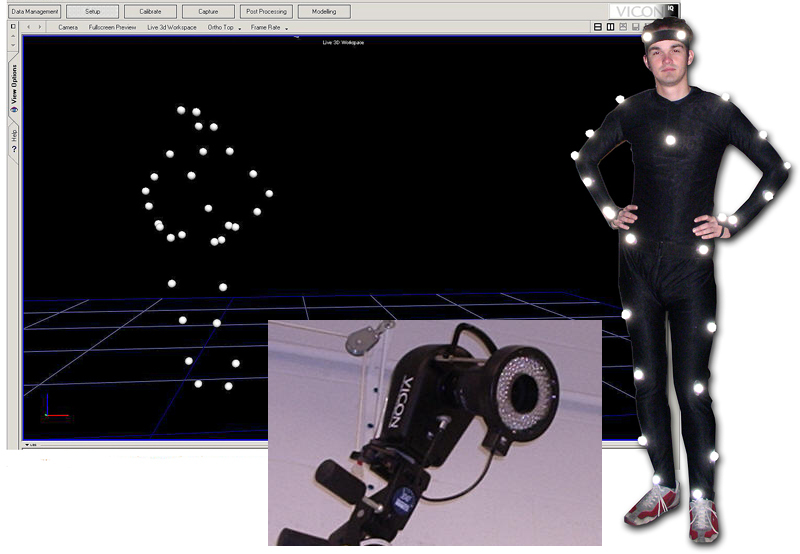
\includegraphics[width=1.5in]{imgs/viconMotionCapture.jpg}}
\end{columns}
\end{frame}

\begin{frame}
\frametitle{Overlays with {\tt pause}}
\setbeamercovered{dynamic}
Practical \TeX\ 2005\\ \pause
Practical \TeX\ 2005\\ \pause
Practical \TeX\ 2005
\end{frame}

\begin{frame}
\frametitle{Tic-Tac-Toe via {\tt tabular}}
\setbeamercovered{invisible}
{\Huge
\begin{center}
\begin{tabular}{c|c|c}
\onslide<9->{O} & \onslide<8->{X} & \onslide<2->{X} \\ \hline
\onslide<6->{X} & \onslide<3->{O} & \onslide<5->{O} \\ \hline
\onslide<10->{X} & \onslide<7->{O} & \onslide<4->{X}
\end{tabular}
\end{center}
}
\end{frame}


\begin{frame}
\frametitle{Tic-Tac-Toe via Graphics Files}
\setbeamercovered{invisible}
\begin{center}
\multiinclude[format=pdf,width=3in]{imgs/hmm}
\end{center}
\end{frame}
\footnotesize
\frame{\section{Introduzione}
\subsection[Problema]{Problema: segmentazione}
\frametitle{Problema}

\begin{block}{Analisi automatica ed in linea della deambulazione umana}
\begin{itemize}
	\item \textbf{analisi}: estrazione di parametri temporali della deambulazione (\textbf{Segmentazione})
	\item \textbf{automatica}: che funziona senza interventi umani
	\item \textbf{in linea }(\textit{online}): vincolo temporale sulla latenza tra verificarsi di un evento ed il tempo di rilevamento del sistema
\end{itemize}
\begin{columns}
\column{.3\textwidth} \hspace{0.5cm}
%\includegraphics[width=0.7\textwidth]{billeder/circuit} 
\column{.7\textwidth}
\end{columns}
\end{block}
}

%%%%%%%%%%%%%%%%%%%%%%%%%%%%%%%%%%%%%%%%%%%%%%%%%%%%%%%%%%%%%%%%%%%%%%%%%%%%%%%%%%%%%%%%%%%%%%%%%%%%%%%%%%%%%%%%%%%%%%%%%

\frame{\subsection[Soluzione]{Soluzione: Hidden Markov Models (HMM)}
\frametitle{Soluzione: prototipo}

\begin{block}{Logica}
\begin{itemize}
	\item \textbf{Modello stocastico per sequenze temporali della deambulazione}: HMM addestrata su $n$ soggetti 
	\item \textbf{Algoritmo di decodifica in linea}: versione in linea dell'algoritmo di Viterbi  
\end{itemize}
\end{block}

\begin{block}{Hardware}
\begin{columns}
	\column{.6\textwidth}
		\begin{itemize}
			\item \textbf{Acquisizione dati deambulazione}: giroscopio monoassiale contenuto in una \textbf{IMU} (Inertial Measurement Unit) 
			\item \textbf{Posizionamento}: collo del piede ed orientato con l'asse sensibile sul piano mediale-laterale
			\item \textbf{Trasmissione}: comunica dati e riceve comandi via \textit{Bluetooth}
		\end{itemize}
	\column{.35\textwidth}
		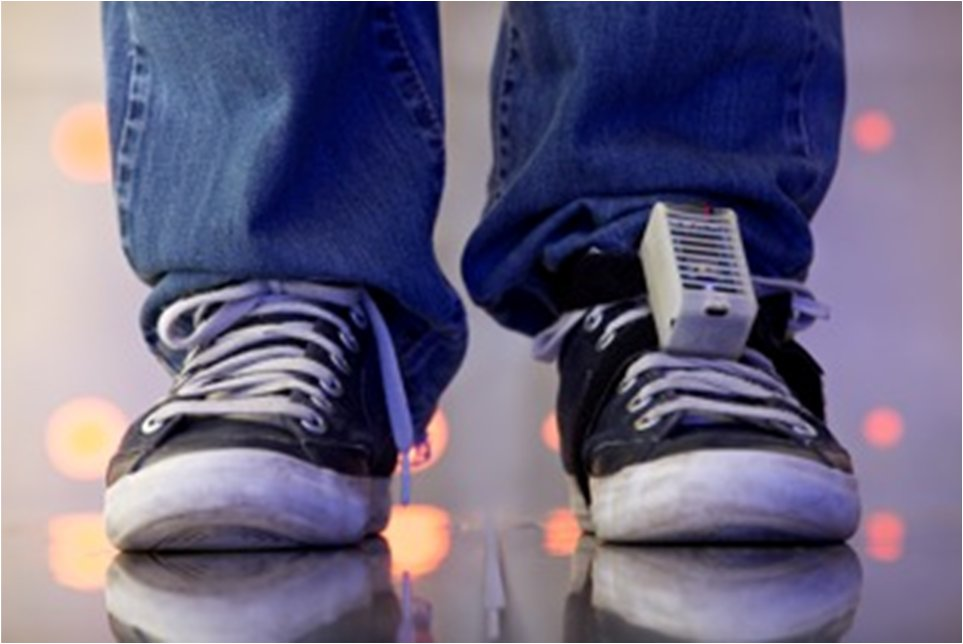
\includegraphics[width=.9\textwidth]{imgs/sensore.jpg}
	\end{columns}
\end{block}

\begin{block}{Software}
\begin{itemize}
	\item \textbf{Controllo, elaborazione e visualizzazione}: \textit{Smartphone} Android\tm
\end{itemize}
\end{block}
}

%%%%%%%%%%%%%%%%%%%%%%%%%%%%%%%%%%%%%%%%%%%%%%%%%%%%%%%%%%%%%%%%%%%%%%%%%%%%%%%%%%%%%%%%%%%%%%%%%%%%%%%%%%%%%%%%%%%%%%%%%
\frame{\subsection{Valutazione}
\frametitle{Valutazione del prototipo}

\begin{block}{Metodo di verifica del funzionamento}
\begin{itemize}
	\item Stima velocit� sistema ideato : $IMUspeed$
	\item Stima velocit� GPS: $GPSspeed$
	\item Confronto: $IMUspeed \approx GPSspeed$ ?
\end{itemize} 
\end{block}


}

\frame{\section{Stato dell'arte}
\subsection[Parametri]{Parametri della deambulazione}
\frametitle{Parametri della deambulazione}

\begin{columns}
\column[b]{.25\textwidth}
\begin{block}{Modellazione}
\begin{enumerate}
	\item Heel Strike
	\item Foot Flat
	\item Heel Off
	\item Toe Off
\end{enumerate}
\end{block}
\column{.8\textwidth}
\begin{figure}
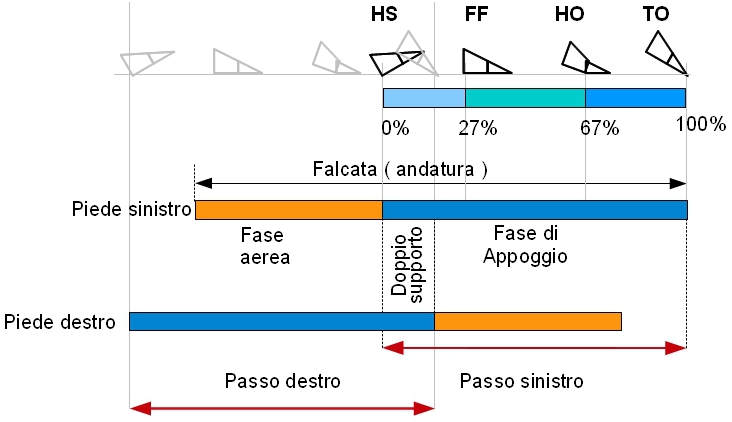
\includegraphics[width=1\textwidth]{imgs/cicloPasso.jpg}\\
\end{figure}

\begin{block}{Valutazione}
\begin{enumerate}
	\item Velocit�: $v\,[m/s]$
	\item Cadenza: $C = num\,passi / s$
\end{enumerate}
\end{block}
\end{columns}
} 


\frame{
\subsection[Letteratura]{Stima dei parametri della deambulazione in letteratura}
\frametitle{Stima dei parametri della deambulazione in letteratura}
\begin{columns}
\column[t]{.5\textwidth}
\begin{block}{Miyazaki (1997) \cite{unrestrained_measurement_stride_length_gyr}}
\textbf{Strumento}: Giroscopio uniassiale \\
\textbf{Posizione}: coscia\\
\textbf{Metodo}: integrazione velocit� angolare
\end{block}
\column[t]{.5\textwidth}
\begin{block}{Aminian et al.(2002) \cite{spatio_temporal_params_gait_gyr}}
\textbf{Strumento}: 2 Giroscopi\\
\textbf{Posizione}: coscia e stinco\\
\textbf{Modello}: modello biomeccanico a pendolo invertito della gamba\\ 
\textbf{Metodo}: basato sulle trasformate \textit{Wavelet}
\end{block}
\end{columns}

\begin{columns}
\column{.5\textwidth}

	\begin{block}{Sabatini et al (2005) \cite{walking_features_from_inertials}}
	\textbf{Strumento}:  1 Giroscopio monoassiale, 2 accelerometri biassiali\\
	\textbf{Posizione}: collo del piede \\
	\textbf{Metodo}: basato su soglie (\textit{threshold-based})
	\end{block}
\column{.5\textwidth}
%	\footnotesize{
%	\begin{table}%
%%	\centering
%	\rowcolors{1}{RoyalBlue!20}{RoyalBlue!5}
%	\begin{tabular}{c|l l}
%	\textbf{E} & \multicolumn{2}{l} {\textbf{regola}}\\
%	%\hline
%	\hline
%	$t_{HS}$ & $ \omega_k \leq 0 $ e $ min_1 \leq  \omega_k$ & $\displaystyle\max_{\forall k}|\widetilde{\omega_k} - \omega_k|$\\
%	%\hline
%	$t_{FF}$ & $|\omega_k|\geq  50$�/s&\\
%	%\hline
%	$t_{HO}$ & $|\omega_k|\geq  50$�/s &\\
%	%\hline
%	$t_{FO}$ & $\omega_k = 0$ & se $\omega$ � diventato positivo \\
%	&\multicolumn{2}{l}{e cresce fino a max.}\\
%	\end{tabular}
%	%\caption{Regole basate sulle soglie (\textit{threshold based}) mediante le quali vengono ricavati gli eventi che delimitano le 4 fasi del cammino \cite{walking_features_from_inertials}.}
%	%\label{tab:regole_threshold_eventi}
%	\end{table}
%	}

\begin{block}{Pfau et al (2008) \cite{stride_segmentation_technique_hmm}}
\textbf{Strumento}:  1 accelerometro triassiale, 1 giroscopio triassiale, un magnetometro\\
\textbf{Posizione}: dorso e torace \\
\textbf{Modello}: HMM per la segmentazione del galoppo\\
\end{block}

\end{columns}
} 

%\frame{
%\frametitle{Materiali e Metodi per la stima dei parametri della deambulazione}
%\begin{block}{Aminian et al.(2002) \cite{spatio_temporal_params_gait_gyr}}
%\textbf{Strumento}: 2 Giroscopi\\
%\textbf{Posizione}: coscia e stinco\\
%\textbf{Modello}: modello biomeccanico a pendolo invertito della gamba\\ 
%\textbf{Metodo}: basato sulle trasformate \textit{Wavelet}
%\end{block}
%} 

%\frame{
%\begin{figure}
%\frametitle{Materiali e Metodi per la stima dei parametri della deambulazione}
%\begin{block}{Sabatini et al (2005) \cite{walking_features_from_inertials}}
%\textbf{Strumento}:  1 Giroscopio monoassiale, 2 accelerometri biassiali\\
%\textbf{Posizione}: collo del piede \\
%\textbf{Metodo}: basato su euristiche (\textit{threshold-based})
%\end{block}
%\centering
%\end{figure}
%\begin{table}%
%\centering
%\begin{tabular}{c|l p{4cm}}
%\textbf{Evento} & \multicolumn{2}{c} {\textbf{regola}}\\
%%\hline
%\hline
%$t_{HS}$ & $ \omega_k \leq 0 $ e $ min_1 \leq  \omega_k$ & $\displaystyle\max_{\forall k}|\widetilde{\omega_k} - \omega_k|$\\
%%\hline
%$t_{FF}$ & $|\omega_k|\geq  50$�/s&\\
%%\hline
%$t_{HO}$ & $|\omega_k|\geq  50$�/s &\\
%%\hline
%$t_{FO}$ & $\omega_k = 0$ & se $\omega$ da negativo � diventato positivo e cresce fino al suo valore massimo.\\
%\end{tabular}
%%\caption{Regole basate sulle soglie (\textit{threshold based}) mediante le quali vengono ricavati gli eventi che delimitano le 4 fasi del cammino \cite{walking_features_from_inertials}.}
%%\label{tab:regole_threshold_eventi}
%\end{table}
%} 



%\frame{
%
%\frametitle{HMM per l'analisi della deambulazione}
%\begin{block}{Pfau et al (2008) \cite{stride_segmentation_technique_hmm}}
%\textbf{Strumento}:  3 accelerometri triassiali, 1 giroscopio triassiale, un magnetometro\\
%\textbf{Posizione}: dorso e torace \\
%\textbf{Modello}: HMM per la segmentazione del galoppo\\
%\textbf{Metodo}:
%\end{block}
%\centering
%%\includegraphics[width=0.65\textwidth]{billeder/poly-florida}
%\end{figure}
%}  

\frame{
\section{Lavoro}
\subsection[Modello]{Parte I. Modellazione della deambulazione}
\frametitle{Raccolta e morfologia dei dati}
\scriptsize{
\begin{table}[htbp]
	\centering
	\rowcolors{1}{RoyalBlue!20}{RoyalBlue!5}
	\begin{tabular}{l|c}
			Attivit�& cammino \\
			Soggetti& $6$ \\
			Velocit�& $\{3,4,5,6,7\}\,km/h$\\
			Durata& $2\, minuti$ per attivit�\\
			Strumenti & IMU, Vicon, tappeto rullante\\
			Luogo& Laboratorio\\
			Dati raccolti & valori giroscopio monoassiale\\
			Freq. camp & $100\, Hz$
		\end{tabular}
	\label{tab:TabellaRiassuntivaRaccoltaDati}
\end{table}
}



\begin{figure}
\centering
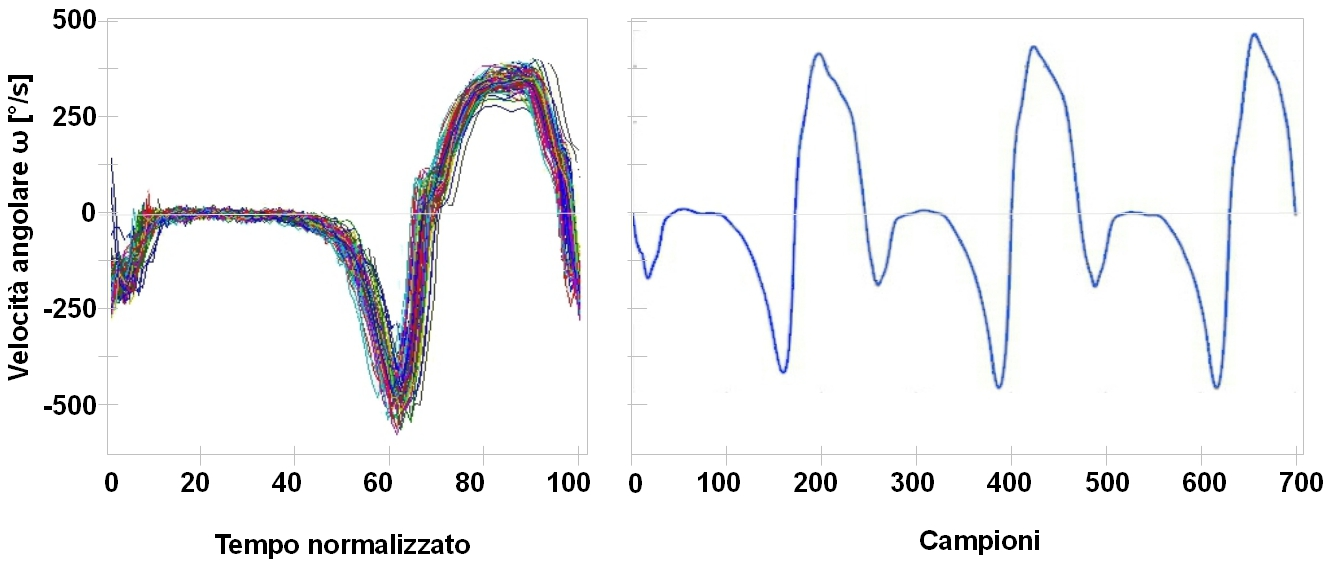
\includegraphics[width=.95\textwidth]{imgs/gyroSignal.jpg}
\end{figure}
} 





\frame{
\begin{figure}
%\frametitle{Parte I. HMM per l'analisi della deambulazione}
\frametitle{HMM per l'analisi della deambulazione}
\centering
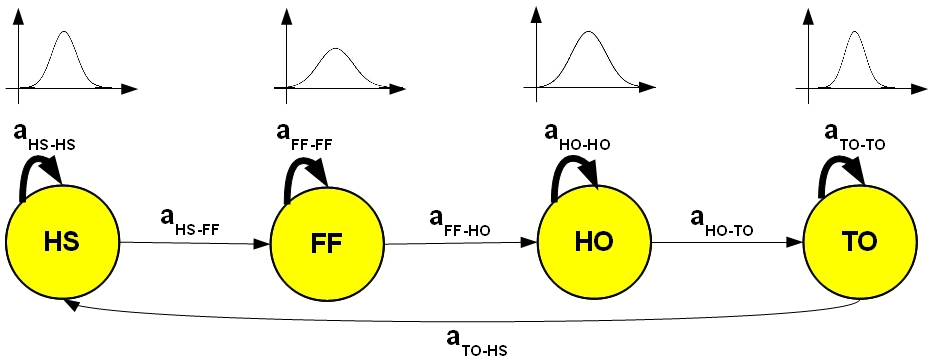
\includegraphics[width=.95\textwidth]{imgs/HMM.jpg}
\end{figure}
\begin{block}{HMM minimale}	
\begin{itemize}
\begin{columns}
\column{.4\textwidth}
	\item $S = \{HS, FF, HO, TO\}$
	\item Sinistra-Destra ciclico 
		\[
			a_{ij} > 0 \Leftrightarrow \left\{
			\begin{array}{l}
				j = i \\
				j = i+1 \\
				i = N \;\text{e}\; j = 1
			\end{array}
		\]

\column{.5\textwidth}
	\item Emissioni gaussiane monovariate $b_j(x) = \mathcal{N}(x,\mu_j,\sigma_j) = \frac{1}{\sigma_j\sqrt{2\pi}}\textbf{e} ^{-\frac{(x-\mu_j)^2}{2\sigma_j^2}}$
	\end{columns}
\end{itemize}
\end{block}
}  




\frame{
\frametitle{Addestramento e validazione modello (1/2): etichettamento}
\begin{columns}[c]
\column{.4\textwidth}
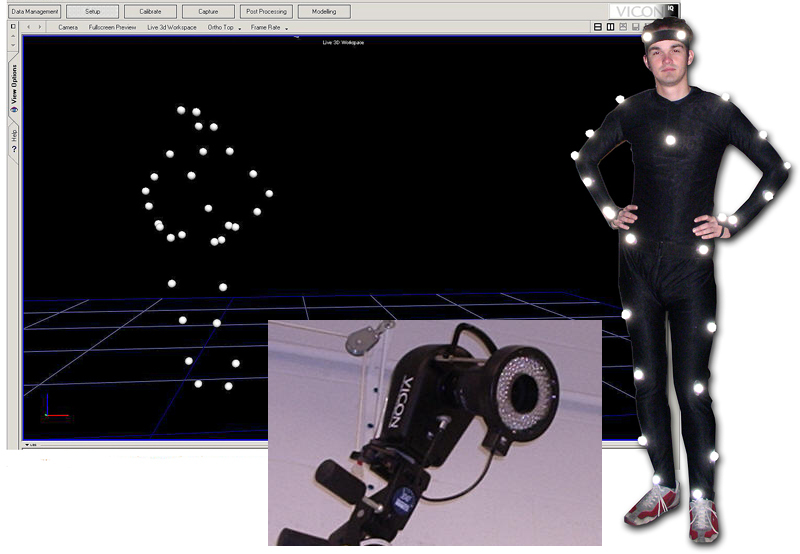
\includegraphics[width=1\textwidth]{imgs/viconMotionCapture.jpg}
\column{.7\textwidth}
\centering
	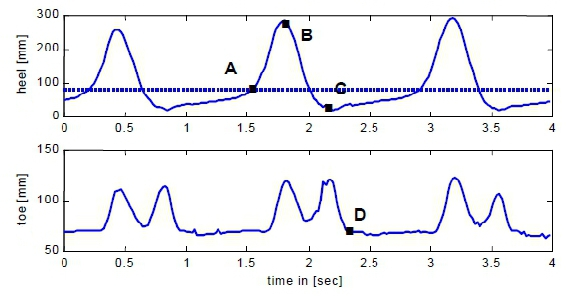
\includegraphics[width=1\textwidth]{imgs/ViconMeasurementsPappas.jpg}


\end{columns}
\begin{block}
\tiny{
\begin{itemize}
	\item $\pi_i = N_i/N_{tot}$
	\item $a_{ij} = $ 
		$
			 \left\{
			\begin{array}{l}
				C/N_i   \quad  \text{se}\quad j = (i+1)\%Q \quad C \,\text{cicli deambulazione nel \textit{Training Set}}\\
				1- C/N_i\quad  \text{se} \quad j = i\\
				0       \quad  \text{altrimenti}
			\end{array}
	$
	\item $b_i(\Omega(t))=$
				$\left\langle \mu_i = \dfrac{1}{N_i} \displaystyle \sum_{t=1}^T{\Omega(t)},\quad
				\sigma_i = \sqrt{\dfrac{1}{N_i -1}\displaystyle \sum_{t=1}^T({\Omega(t)-\mu_i})^2} \right\rangle$
\end{itemize}
}
\end{block}
} 

 
\frame{
\frametitle{Addestramento e validazione modello (2/2): \textit{leave} \textit{one} \textit{subject} \textit{out} \textit{cross} \textit{validation}}
\begin{block}{Validazione della capacit� di generalizzazione del modello}
\centering
	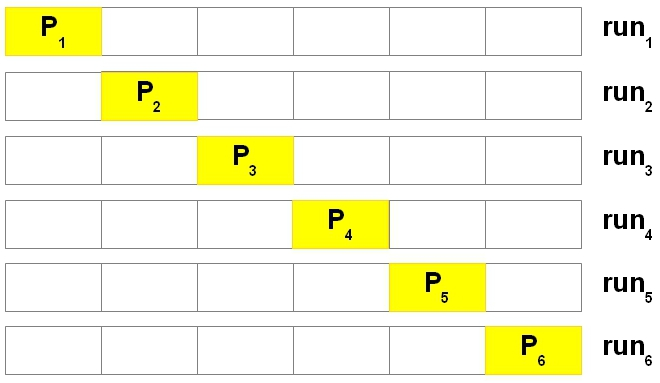
\includegraphics[width=.7\textwidth]{imgs/LOOCV.jpg}
\end{block}
}

\frame{
%
\frametitle{La segmentazione}
\begin{block}{Algoritmo di Viterbi}
Data $\left\langle HMM, O\right\rangle$, la decodifica restituisce sequenza pi� probabile di stati $S^*$. 
\begin{enumerate}
	\item Fase \textit{Forward}: costruzione di sequenze parziali a probabilit� massima
	\item Fase \textit{Backtracking}: calcolo a ritroso della sequenza pi� probabile
\end{enumerate}
\end{block}

\begin{columns}
\column{.5\textwidth}
\begin{block}{Problema}
\textit{Backtracking} non in linea
\end{block}
\column{.5\textwidth}
\begin{block}{Soluzione}
\textit{Short-Time Viterbi} Bloit-Rodet 2008 \cite{short_time_viterbi_online_hmm_deconding}\\
\end{block}
\end{columns}

\begin{block}{Funzionamento Viterbi in linea}
\begin{enumerate}
	\item creazione di una finestra temporale $[a,b]$ 
	\item applicazione Viterbi solo fase \textit{Forward} 
	\item \textit{Backtracking} da ciascuno stato finale 
	\item le sequenze da $a$ fino a $\tau \;(\tau \leq b)$ combaciano $\Rightarrow$ segmentazione 
	\begin{itemize}
		\item spostamento finestra $a = a + \tau$ e $b = a + 1$ e fase (2)
	\end{itemize}
	\item altrimenti
	\begin{itemize}
		\item allargamento finestra $b = b + 1$ e fase (2)
	\end{itemize}
\end{enumerate}
\end{block}
}


%%%%%%%%%%%%%%%%%%%%%%%%%%%%%%%%%%%%%%%%%%%%%%%%%%%%%%%%%%%%%%%%%%%%%%%%%%%%%%%%%%%%%%%%%%%%%%%%%%%%%%%%%%%%%%%%%%%%%%%%%
%%%%%%%%%%%%%%%%%%%%%%%%%%%%%%%%%%%%%%%%%%%%%%%%%%%%%%%%%%%%%%%%%%%%%%%%%%%%%%%%%%%%%%%%%%%%%%%%%%%%%%%%%%%%%%%%%%%%%%%%%
\frame{\subsection[Android app]{Parte II. Applicazione Android\tm}
\frametitle{Architettura dell'applicazione}
\begin{center}
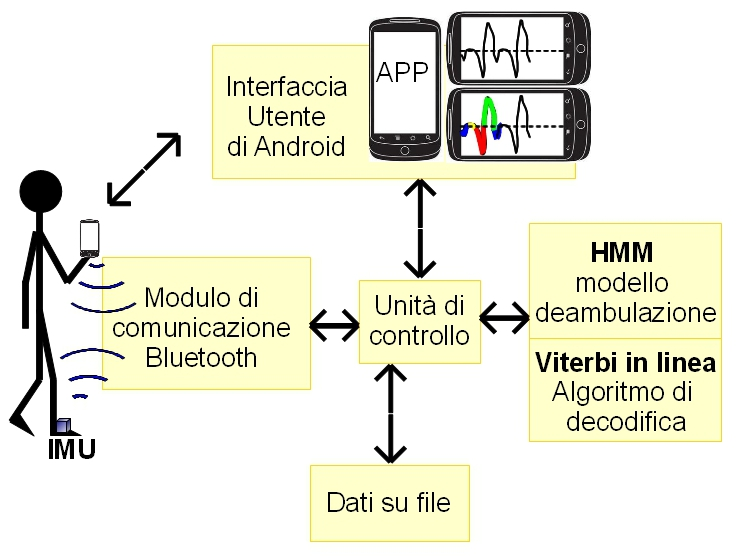
\includegraphics[width=.8\textwidth]{imgs/ArchitetturaProgramma.jpg}
\end{center}
} 


\frame[containsverbatim]{
\frametitle{Interfaccia utente}

\begin{center}
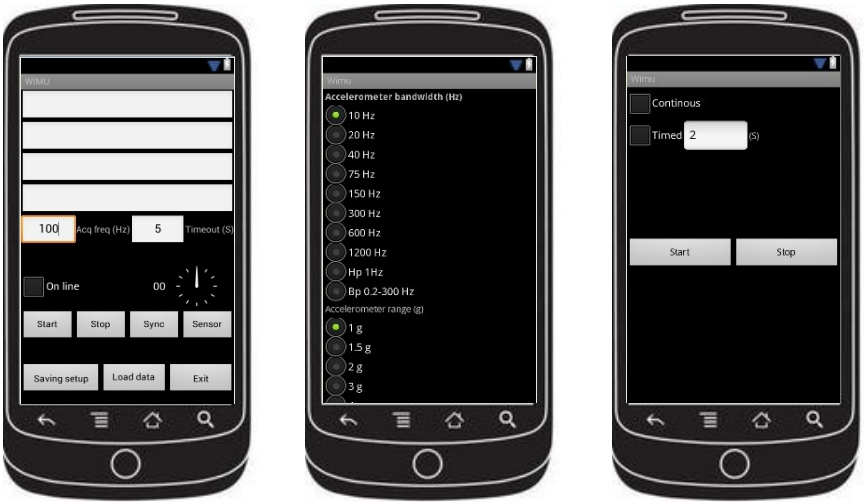
\includegraphics[width=.8\textwidth]{imgs/UI.jpg}
\end{center}
\begin{columns}
\column{.45\textwidth}
\begin{block}{Criteri di programmazione}
\begin{itemize}
	\item semplicit�
	\item classe \verb|Activity|
	\item programmazione a eventi
\end{itemize}
\end{block}
\column{.5\textwidth}
\put(-20,0){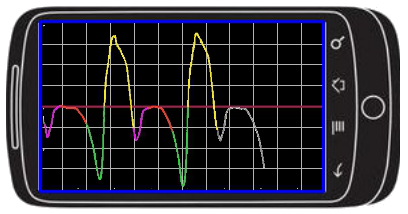
\includegraphics[width=.9\textwidth]{imgs/SegmentationAndroid.png}}
\end{columns}
}


\frame[containsverbatim]{
%\frametitle{Parte II. Applicazione Android\tm: gestione processi}
\frametitle{Gestione processi, Comunicazione}
\begin{block}{Thread e Android: massima reattivit� (5s di blocco tollerato)}
\begin{itemize}
	\item \textit{UI-thread} (main) delega operazioni lunghe o potenzialmente bloccanti. 
	\item Asincrono: un \textit{task} viene eseguito da \textit{worker thread} ed il risultato viene pubblicato sullo \textit{UI-thread} mediante \verb|Handler|
%	A Handler allows you to send and process Message and Runnable objects associated with a thread's MessageQueue. Each Handler instance is associated with a single thread and that thread's message queue. When you create a new Handler, it is bound to the thread / message queue of the thread that is creating it -- from that point on, it will deliver messages and runnables to that message queue and execute them as they come out of the message queue.

	
\end{itemize}
\end{block}

\begin{block}{Comunicazione}
\begin{itemize}
	\item \verb|Intent|: sistema di messaggistica per \verb|Activity| ed altri componenti
	\item \verb|Application|: stato globale dell'applicazione
\end{itemize}
\end{block}
}

\frame{
\frametitle{Implementazione HMM e Viterbi in Java - Android\tm}
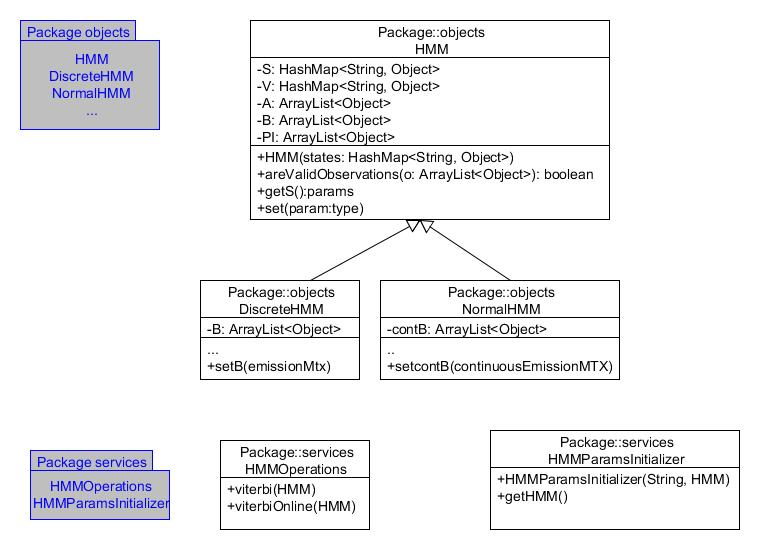
\includegraphics[width=.95\textwidth]{imgs/HMMuml.jpg}\\
}


\frame{
\subsection{Parte III. Valutazione}
%\frametitle{Parte III. Valutazione delle prestazioni del sistema}
\frametitle{Valutazione delle prestazioni del sistema}
\begin{columns}
\column{.5\textwidth}
%\putat{100}{-110}{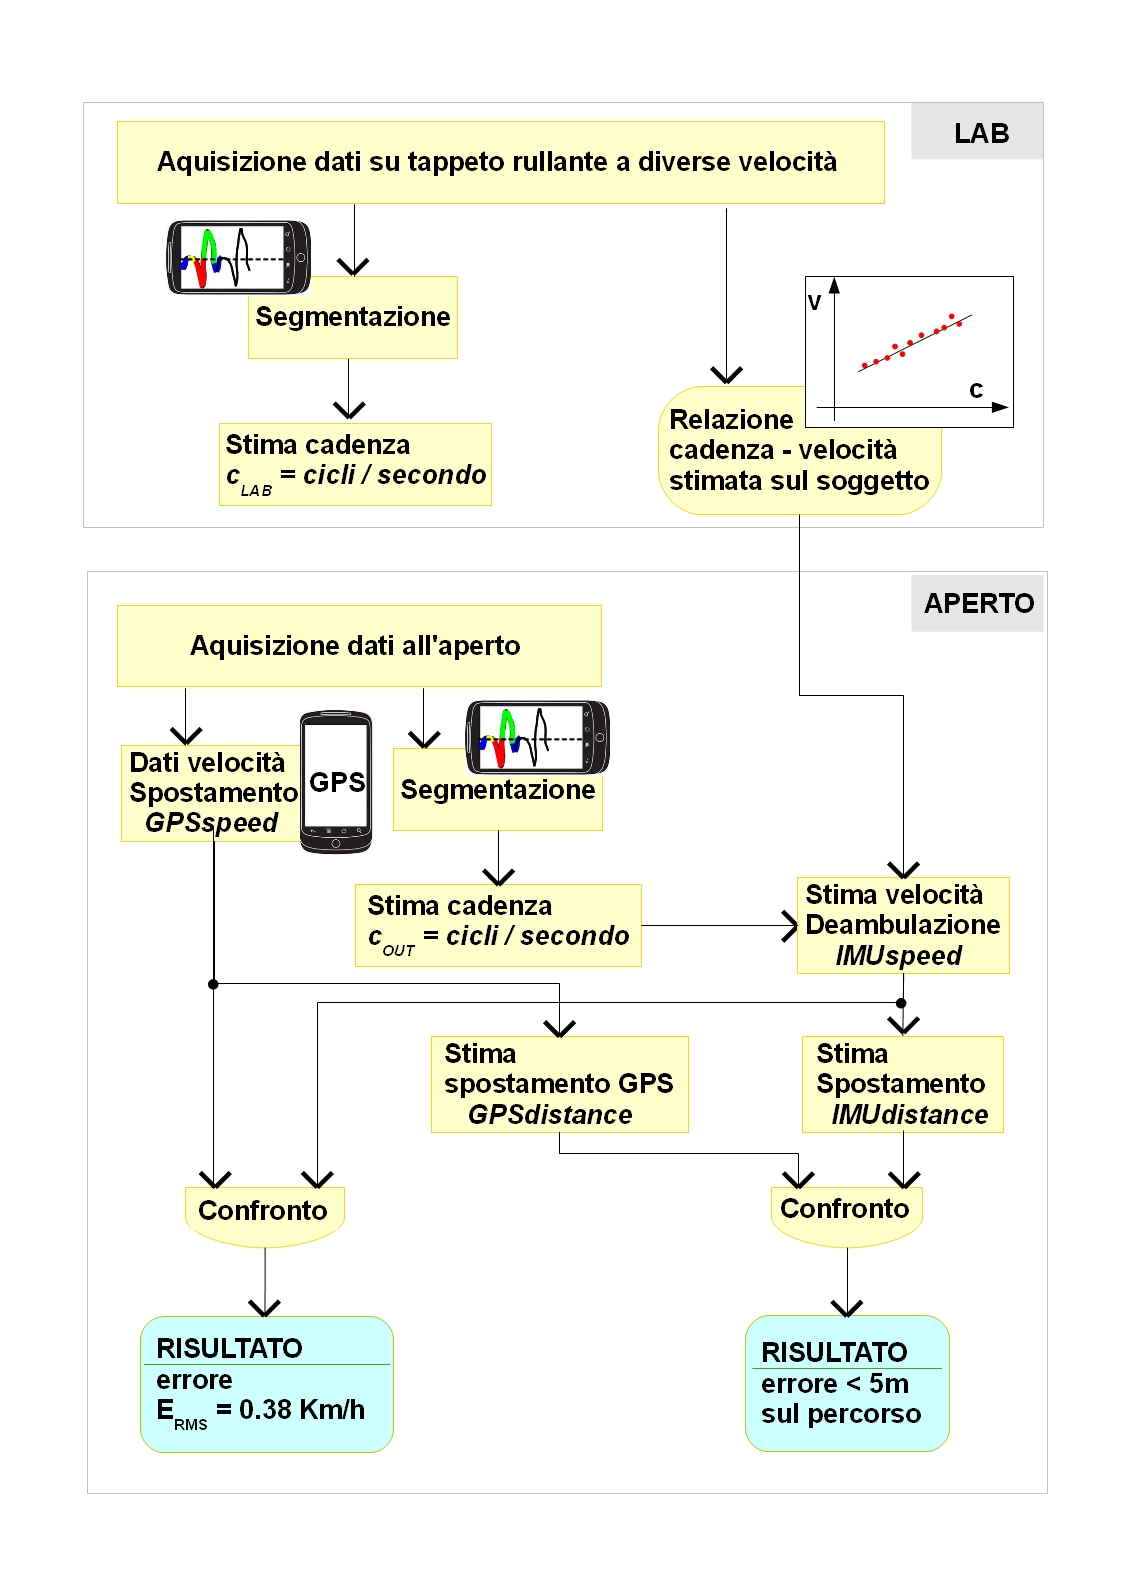
\includegraphics[width=1\textwidth]{imgs/ValutazionePrestazioniSistema.jpg}}\\
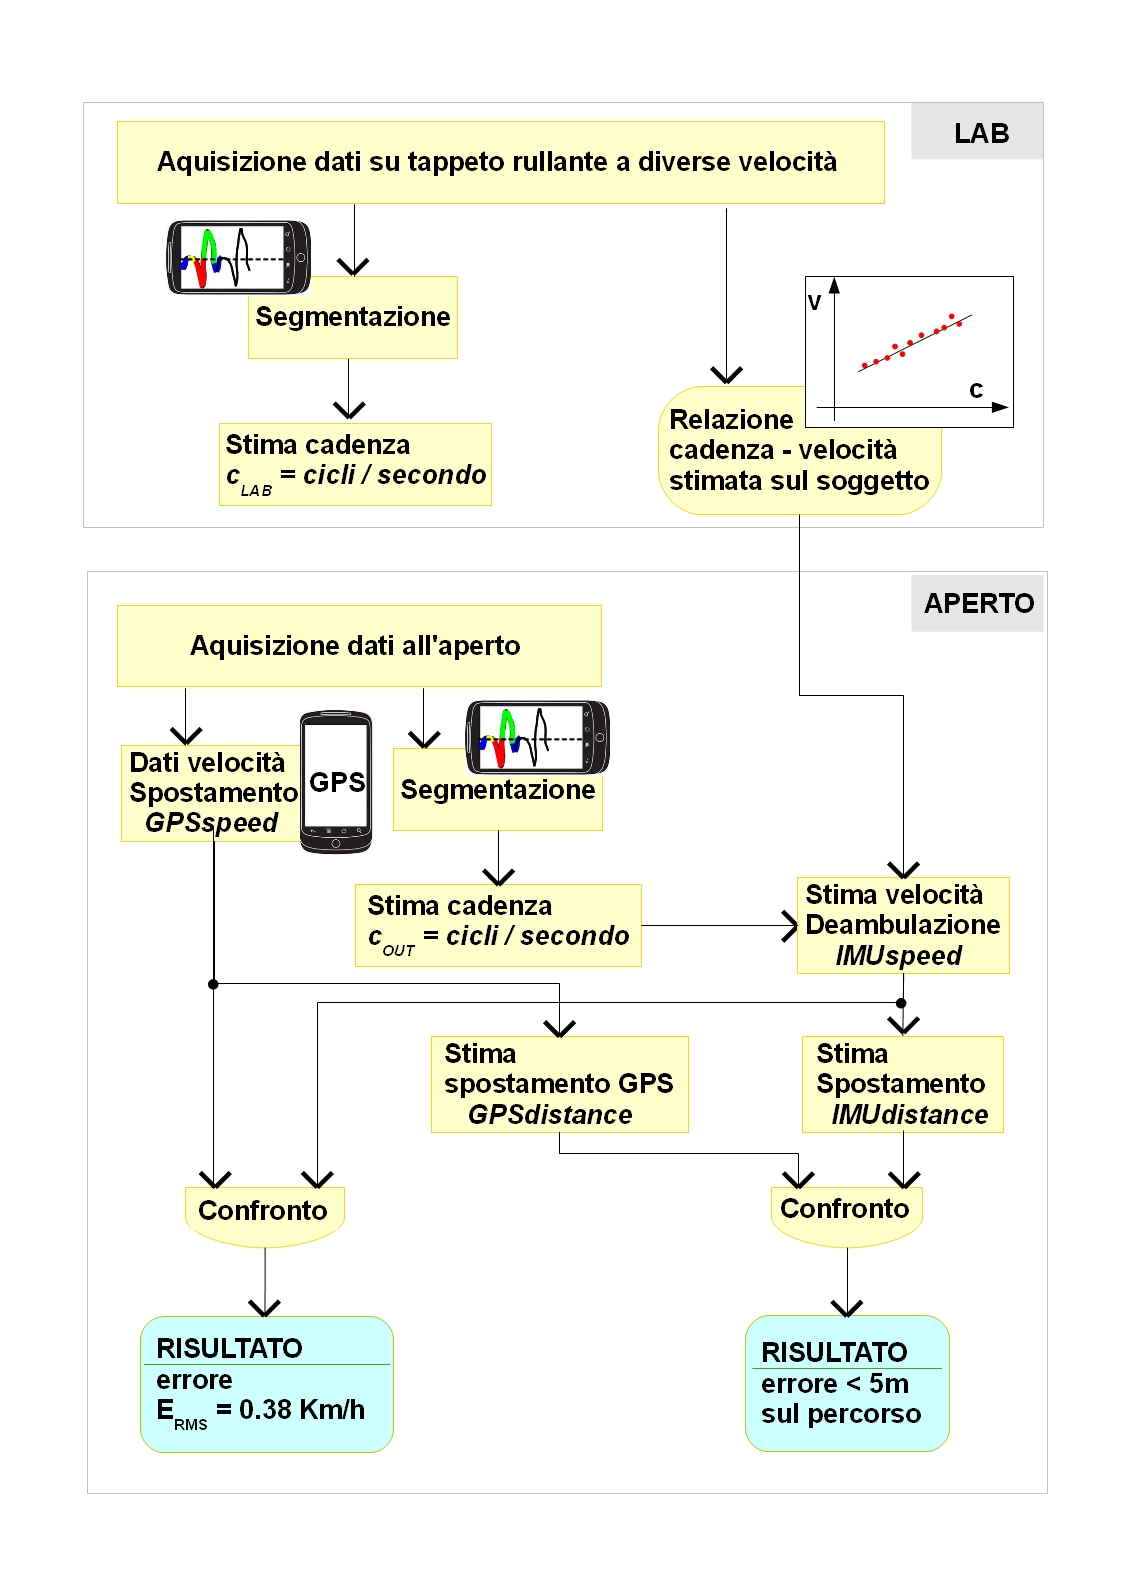
\includegraphics[width=1\textwidth]{imgs/ValutazionePrestazioniSistema.jpg}\\
\column{.5\textwidth}

\tiny{
\begin{table}[htbp]
		\centering
		\rowcolors{1}{RoyalBlue!20}{RoyalBlue!5}
		\begin{tabular}{l|c}
				\textbf{Attivit�}& cammino\\
				\textbf{Soggetti}& $1$\\
				\textbf{Velocit�}& $\{2,3,4,5,6,7,8\}\, km/h$\\
				\textbf{Durata}& $1:30\,minuti$  per attivit�\\
				\textbf{Strumenti} & IMU, Smartphone, tappeto rullante\\
				\textbf{Luogo}& Laboratorio\\
				\textbf{Dati raccolti} & valori giroscopio segmentati\\
				\textbf{Freq. camp.} & $100\,Hz$\\
			\end{tabular}
	\end{table}
}

\begin{flushleft}
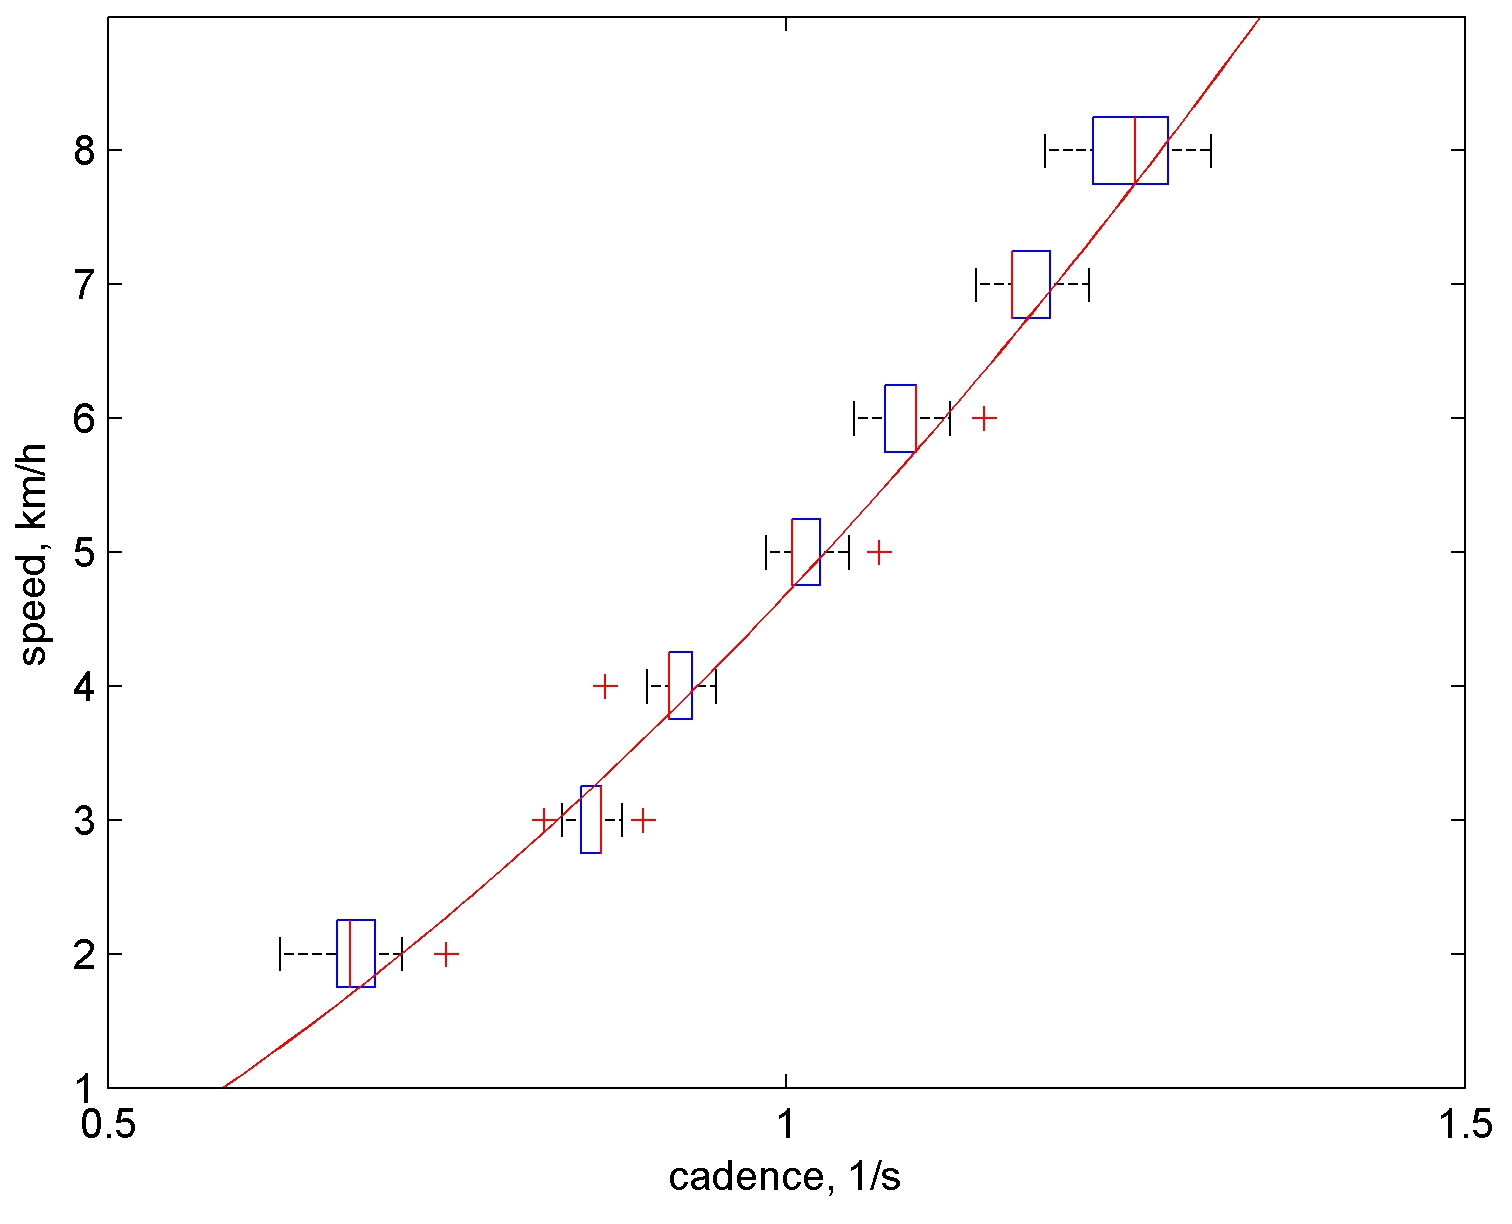
\includegraphics[width=1\textwidth]{imgs/cadVSspeed_boxplot.jpg}
\end{flushleft}

	
\end{columns}
}

\section{Risultati}




\frame{\frametitle{Risultati: stima della velocit�}
\centering
\begin{columns}
\column{.5\textwidth}
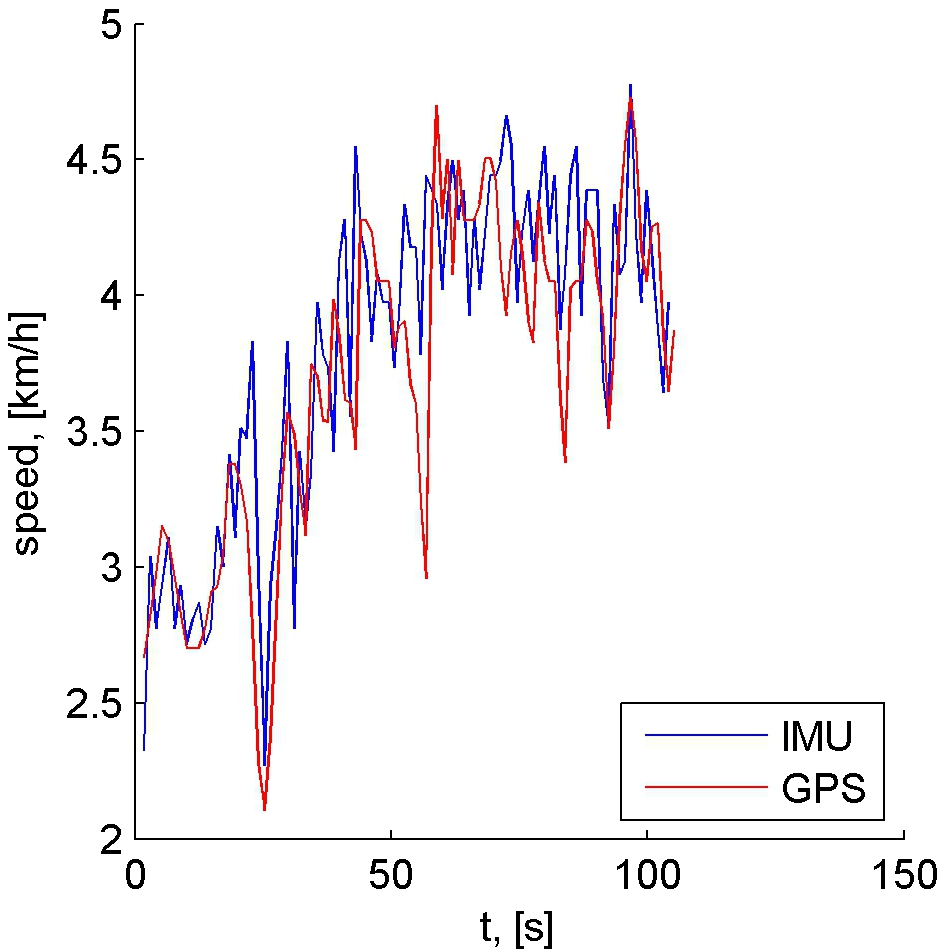
\includegraphics[width=1\textwidth]{imgs/speedSVRs.jpg}
\column{.5\textwidth}
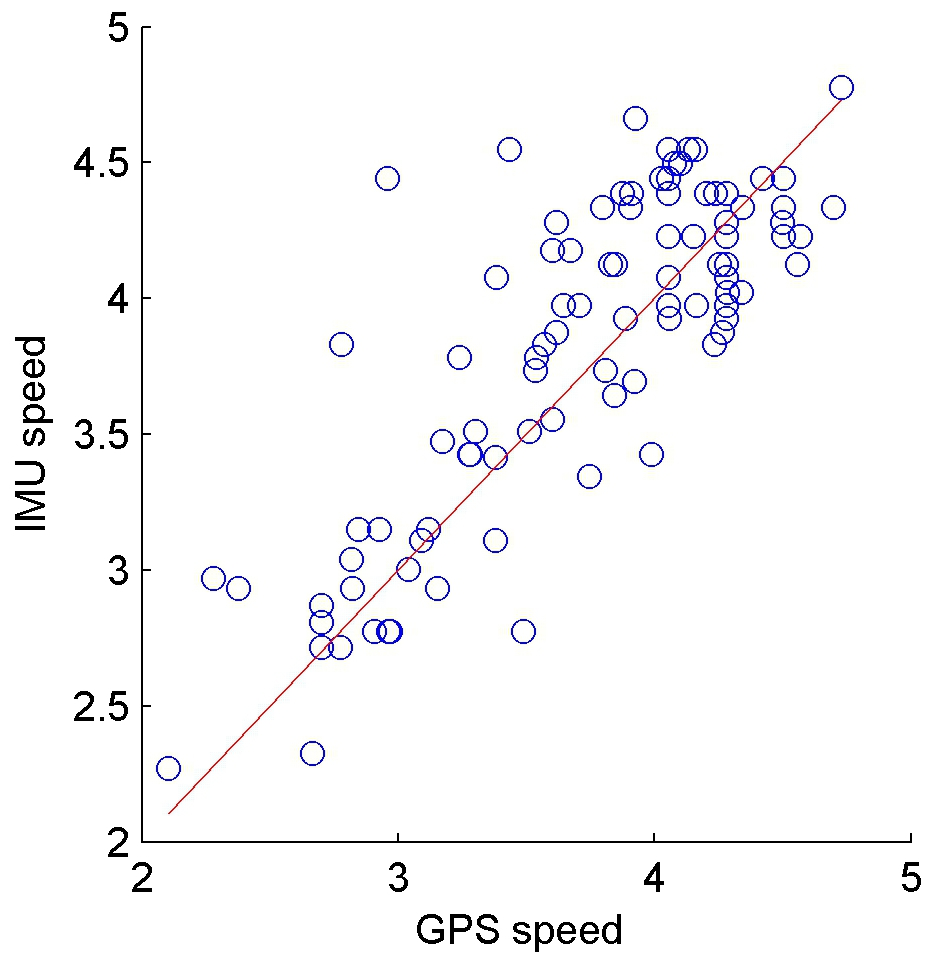
\includegraphics[width=1\textwidth]{imgs/speedSVRd.jpg}
\end{columns}
}

\frame{\frametitle{Risultati: stima della distanza}
\centering
\begin{columns}
\column{.5\textwidth}
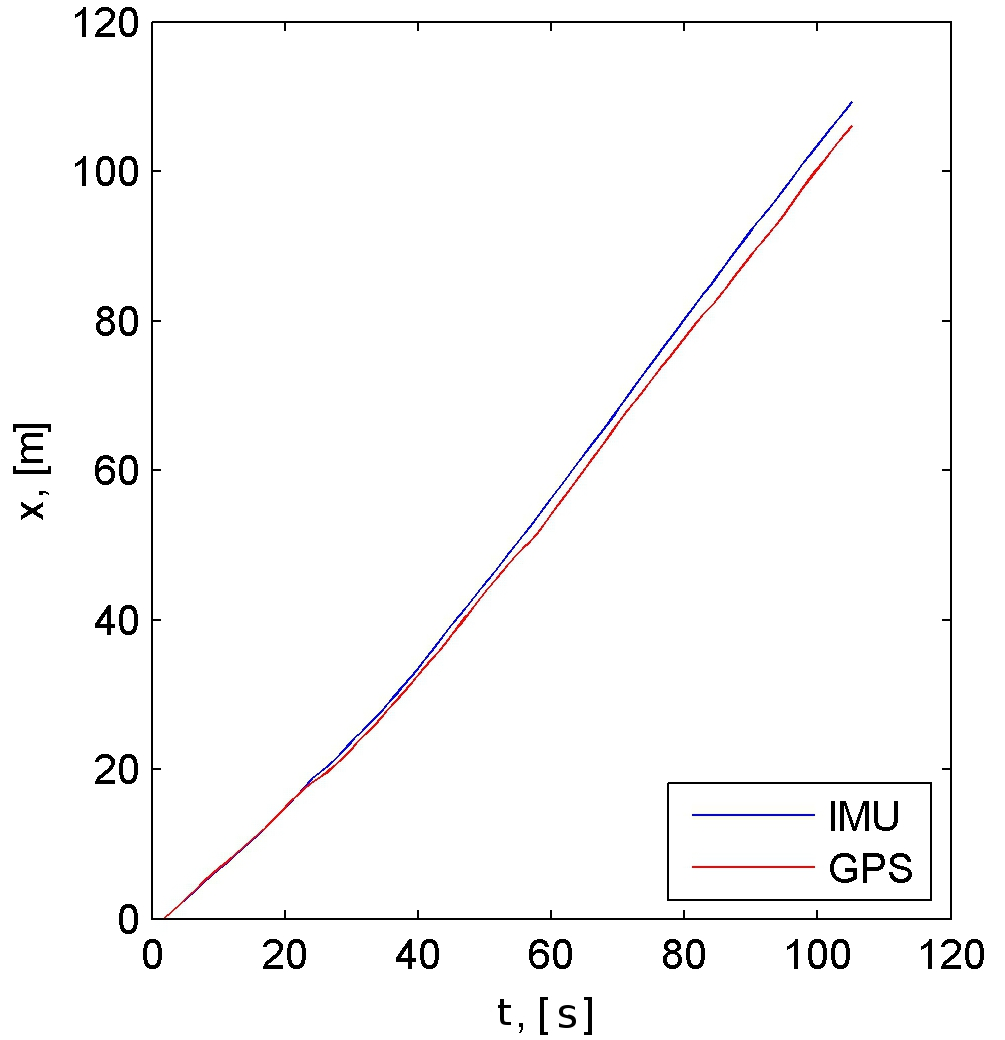
\includegraphics[width=1\textwidth]{imgs/displSVRs.jpg}
\column{.5\textwidth}
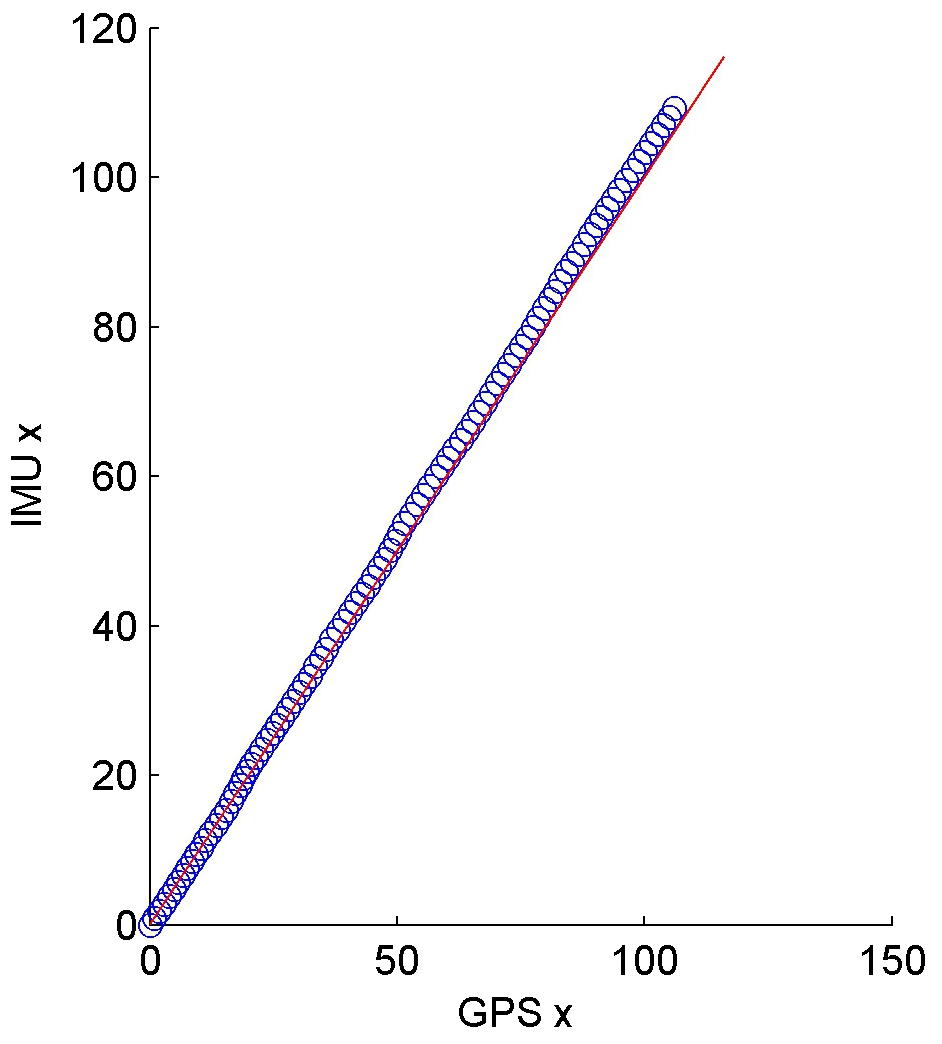
\includegraphics[width=1\textwidth]{imgs/displSVRd.jpg}
\end{columns}
}

\section{Conclusioni}

\frame{
\frametitle{Conclusioni}
\begin{block}{Successi}
	\begin{itemize}
		\item � in grado di segmentare in linea la deambulazione
		\item in grado di generalizzare 
		\item hardware minimale: \textit{Smartphone} e singolo giroscopio
	\end{itemize}
\end{block}
\begin{block}{Possibile applicazione}
Spia di deambulazione anormale
\end{block}

\begin{block}{Sviluppi futuri}
\begin{itemize}
	\item Sperimentazione su larga scala: addestramento e verifica
	\item Riconoscimento di attivit� mediante gerarchia di HMM 
\end{itemize}
\end{block}


}
%\frame{\frametitle{Conclusioni}
%\begin{block}{Conclusioni: Limiti del lavoro}
%\begin{itemize}
%	\item addestramento solo su 6 individui
%	\item fase di verifica poco tempo e individui
%	\item ...
%\end{itemize}
%\end{block}
%%}
%\frame{\frametitle{Possibili applicazioni}
%\begin{block}{Sostituzione temporanea GPS}
%Dispositivo per la navigazione personale basato su dati inerziali: il GPS pu� incappare in problemi di assenza di segnale, il sistema pu� subentrare nella misurazione della distanza per brevi periodi di tempo ed essere sostituito dal GPS, quando il segnale � nuovamente disponibile.\\ 
%Funziona anche al chiuso.
%\end{block}
%
%}


\frame{
\centering
\fontsize{50pt}{60pt}\selectfont
\begin{block}

\begin{center}
Grazie!
\end{center}
\end{block}
}
\appendix

\beginbackup 


\frame{
%\subsection{Parte I}
%\frametitle{Parte I. HMM per l'analisi della deambulazione: definizione}
\frametitle{Definizione di un'Hidden Markov Model (HMM)}
\begin{columns}
\column{.6\textwidth}

	\begin{figure}
	\centering
	  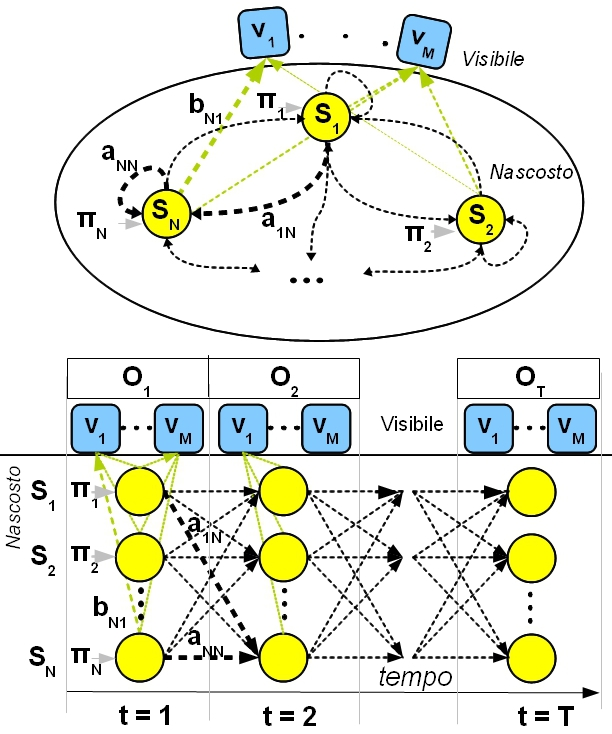
\includegraphics[width=.9\textwidth]{imgs/descreteMarkovProcesses2.jpg}	
	\end{figure}

\column{.5\textwidth}

%	\tiny{
	HMM $= <N, M, \mathbf{A}, \mathbf{B}, \mathbf{\pi}>$
dove: 

\begin{enumerate}
	\item $N = |S|$: stati nascosti
	\item $M = |V|$:  alfabeto osservazione
	\item $\mathbf{A}\{a_{ij}\}$: probabilit� di transizione 
				$a_{ij} = \wp[q_t = S_j | q_{t-1} = S_i]$
	\item $\mathbf{B}$ :probabilit� di emissione
				$b_j(k) = \wp[v_k \; \text{all'istante } t | q_t = s_j] $
	\item $\mathbf{\pi}$: probabilit� a priori
				$\pi_i = \wp(q_1 = S_i)$
				
\end{enumerate}

\end{columns}
%}

}



\frame{
%\subsection[Segmentazione]{Parte I. Segmentazione dei dati giroscopici relativi alla deambulazione}
\frametitle{La segmentazione: algoritmo di Viterbi}
%\begin{algorithm} 
%\caption{Viterbi}
%\label{alg:viterbi}                                                  
\begin{columns}
\column{.5\textwidth}
Viterbi
\begin{algorithmic}[1]                    
\STATE{}\COMMENT{\textit{Inizializzazione}}
\FOR {$i = 0$ to $N$}
	\STATE {$\delta_{i,1} = \pi_i b_i(o_1)$}
	\STATE {$\psi_{i,1} = 0$}
\ENDFOR
\STATE{}\COMMENT{\textit{Iterazione}}
\FOR{$t = 2$ to $T$}
	\FOR{$i = 1$ to $N$} 
		\STATE $ \delta_{i,t}=\displaystyle\max_{1\leq j \leq N} [\delta_{j,t-1}a_{j,i}]* b_i(o_i)$
		\STATE $ \psi_{i,t}=\displaystyle\arg \max_{1\leq j \leq N} [\delta_{j, t-1}a_{j,i}]$
	\ENDFOR
\ENDFOR
\STATE{}\COMMENT{\textit{Terminazione}}
\STATE $P* = \displaystyle \max_{1\leq i \leq N} [\delta_{i,T}]$
\STATE $q_T* = \displaystyle \arg \max_{1\leq i \leq N} [\delta_{i,T}]$
\STATE{}\COMMENT{Backtracking}
\FOR{$t=T-1$ to $1$}
	\STATE{$q*_t=\psi_{q*_{t+1},t+1}$}
\ENDFOR
\end{algorithmic}
%\end{algorithm}
\column{.5\textwidth}
\end{columns}
}
\endbackup
%


%\begin{enumerate}
%	\item $N$:  stati nascosti
%	\item $M = |V|$: alfabeto osservazione
%%	\item $\mathbf{A} = \{a_{ij}\}$: probabilit� di transizione \\
%%	\item $N = 4$ , stati $S = \{HS, FF, HO, FO\}$
%%	\item $M = |V|$, valori di osservazione segnale giroscopico 
%	
%
%%	$\omega (^\circ/s)$ $a_{ij} = \wp[q_t = S_j | q_{t-1} = S_i]$
%%		\begin{equation}
%			%\begin{split}
%%			$A = \,& \{a_{ij}\}\; 	
%\item $\mathbf{B} = \{b_j(k)\}$: probabilit� di emissione\\ 
%%			\end{split}
%%		\end{equation}$b_j(k) = \wp[v_k \; \text{all'istante } t | q_t = s_j] $
%%	delle osservazioni $\omega$ di ciascuno stato $S_i$
%%	\begin{equation}
%%\begin{split}
%%$\mathbf{B} = \{b_j(k)\}\;	
%\item $\pi = \{\pi_i\}$: probabilit� a priori \\
%%\end{split}	 
%%\label{eq:emissionMtxDef}
%%\end{equation}	
%%		\begin{equation}
%%	B = b_j(x) = \mathcal{N}(x,\mu_j,\sigma_j) = \frac{1}{\sigma_j\sqrt{2\pi}}\textbf{e} ^{-\frac{(x-\mu_j)^2}{2 \sigma_j^2}}\quad
%%		\text{per} 1 \leq j \leq N \nonumber
%%		\end{equation}$\pi_i = \wp(q_1 = S_i)$\\\vspace{.5cm}
%%	\begin{equation}
%%\begin{split}
%$	\mathbf{\pi} = \{p_i\}\; $1\leq i,j \leq N $ e $1\leq k \leq M$ 
%%\end{split}	
%%\label{eq:prior}
%%\end{equation}
%\end{enumerate}	


\frame{
%\subsection{}
\frametitle{Parte I. HMM per l'analisi della deambulazione: definizione}

\begin{columns}
\column{.6\textwidth}

	\begin{figure}
	\centering
	  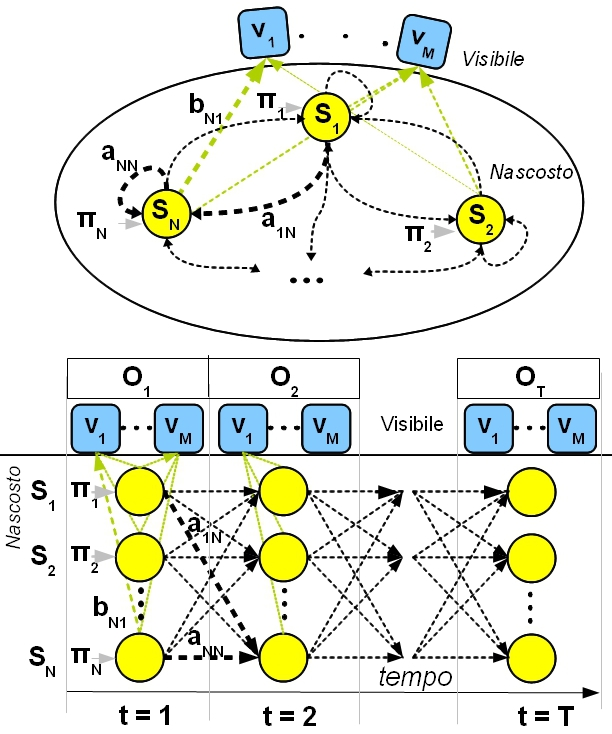
\includegraphics[width=.9\textwidth]{imgs/descreteMarkovProcesses2.jpg}	
	\end{figure}

\column{.5\textwidth}

	\tiny{
	HMM $= <N, M, \mathbf{A}, \mathbf{B}, \mathbf{\pi}>$
dove: 

\begin{enumerate}
	\item $N = |S|$: stati nascosti
	\item $M = |V|$:  alfabeto osservazione
	\item $\mathbf{A}\{a_{ij}\}$: probabilit� di transizione 
				$a_{ij} = \wp[q_t = S_j | q_{t-1} = S_i]$
	\item $\mathbf{B}$ :probabilit� di emissione
				$b_j(k) = \wp[v_k \; \text{all'istante } t | q_t = s_j] $
	\item $\mathbf{\pi}$: probabilit� a priori
				$\pi_i = \wp(q_1 = S_i)$
				
\end{enumerate}

\end{columns}
}

}



%\section{Introduzione}
\section{Stato dell'arte}
\section{Lavoro svolto}
\section{Risultati}
\section{Conclusioni}
\bibliographystyle{IEEEtran}
\bibliography{biblio}
\end{document}